\PassOptionsToPackage{unicode=true}{hyperref} % options for packages loaded elsewhere
\PassOptionsToPackage{hyphens}{url}
%
\documentclass[]{article}
\usepackage{lmodern}
\usepackage{amssymb,amsmath}
\usepackage{ifxetex,ifluatex}
\usepackage{fixltx2e} % provides \textsubscript
\ifnum 0\ifxetex 1\fi\ifluatex 1\fi=0 % if pdftex
  \usepackage[T1]{fontenc}
  \usepackage[utf8]{inputenc}
  \usepackage{textcomp} % provides euro and other symbols
\else % if luatex or xelatex
  \usepackage{unicode-math}
  \defaultfontfeatures{Ligatures=TeX,Scale=MatchLowercase}
\fi
% use upquote if available, for straight quotes in verbatim environments
\IfFileExists{upquote.sty}{\usepackage{upquote}}{}
% use microtype if available
\IfFileExists{microtype.sty}{%
\usepackage[]{microtype}
\UseMicrotypeSet[protrusion]{basicmath} % disable protrusion for tt fonts
}{}
\IfFileExists{parskip.sty}{%
\usepackage{parskip}
}{% else
\setlength{\parindent}{0pt}
\setlength{\parskip}{6pt plus 2pt minus 1pt}
}
\usepackage{hyperref}
\hypersetup{
            pdftitle={Generate Reproducible \& Live HTML and PDF Conference Posters Using RMarkdown},
            pdfborder={0 0 0},
            breaklinks=true}
\urlstyle{same}  % don't use monospace font for urls
\usepackage[margin=1in]{geometry}
\usepackage{color}
\usepackage{fancyvrb}
\newcommand{\VerbBar}{|}
\newcommand{\VERB}{\Verb[commandchars=\\\{\}]}
\DefineVerbatimEnvironment{Highlighting}{Verbatim}{commandchars=\\\{\}}
% Add ',fontsize=\small' for more characters per line
\usepackage{framed}
\definecolor{shadecolor}{RGB}{248,248,248}
\newenvironment{Shaded}{\begin{snugshade}}{\end{snugshade}}
\newcommand{\AlertTok}[1]{\textcolor[rgb]{0.94,0.16,0.16}{#1}}
\newcommand{\AnnotationTok}[1]{\textcolor[rgb]{0.56,0.35,0.01}{\textbf{\textit{#1}}}}
\newcommand{\AttributeTok}[1]{\textcolor[rgb]{0.77,0.63,0.00}{#1}}
\newcommand{\BaseNTok}[1]{\textcolor[rgb]{0.00,0.00,0.81}{#1}}
\newcommand{\BuiltInTok}[1]{#1}
\newcommand{\CharTok}[1]{\textcolor[rgb]{0.31,0.60,0.02}{#1}}
\newcommand{\CommentTok}[1]{\textcolor[rgb]{0.56,0.35,0.01}{\textit{#1}}}
\newcommand{\CommentVarTok}[1]{\textcolor[rgb]{0.56,0.35,0.01}{\textbf{\textit{#1}}}}
\newcommand{\ConstantTok}[1]{\textcolor[rgb]{0.00,0.00,0.00}{#1}}
\newcommand{\ControlFlowTok}[1]{\textcolor[rgb]{0.13,0.29,0.53}{\textbf{#1}}}
\newcommand{\DataTypeTok}[1]{\textcolor[rgb]{0.13,0.29,0.53}{#1}}
\newcommand{\DecValTok}[1]{\textcolor[rgb]{0.00,0.00,0.81}{#1}}
\newcommand{\DocumentationTok}[1]{\textcolor[rgb]{0.56,0.35,0.01}{\textbf{\textit{#1}}}}
\newcommand{\ErrorTok}[1]{\textcolor[rgb]{0.64,0.00,0.00}{\textbf{#1}}}
\newcommand{\ExtensionTok}[1]{#1}
\newcommand{\FloatTok}[1]{\textcolor[rgb]{0.00,0.00,0.81}{#1}}
\newcommand{\FunctionTok}[1]{\textcolor[rgb]{0.00,0.00,0.00}{#1}}
\newcommand{\ImportTok}[1]{#1}
\newcommand{\InformationTok}[1]{\textcolor[rgb]{0.56,0.35,0.01}{\textbf{\textit{#1}}}}
\newcommand{\KeywordTok}[1]{\textcolor[rgb]{0.13,0.29,0.53}{\textbf{#1}}}
\newcommand{\NormalTok}[1]{#1}
\newcommand{\OperatorTok}[1]{\textcolor[rgb]{0.81,0.36,0.00}{\textbf{#1}}}
\newcommand{\OtherTok}[1]{\textcolor[rgb]{0.56,0.35,0.01}{#1}}
\newcommand{\PreprocessorTok}[1]{\textcolor[rgb]{0.56,0.35,0.01}{\textit{#1}}}
\newcommand{\RegionMarkerTok}[1]{#1}
\newcommand{\SpecialCharTok}[1]{\textcolor[rgb]{0.00,0.00,0.00}{#1}}
\newcommand{\SpecialStringTok}[1]{\textcolor[rgb]{0.31,0.60,0.02}{#1}}
\newcommand{\StringTok}[1]{\textcolor[rgb]{0.31,0.60,0.02}{#1}}
\newcommand{\VariableTok}[1]{\textcolor[rgb]{0.00,0.00,0.00}{#1}}
\newcommand{\VerbatimStringTok}[1]{\textcolor[rgb]{0.31,0.60,0.02}{#1}}
\newcommand{\WarningTok}[1]{\textcolor[rgb]{0.56,0.35,0.01}{\textbf{\textit{#1}}}}
\usepackage{graphicx,grffile}
\makeatletter
\def\maxwidth{\ifdim\Gin@nat@width>\linewidth\linewidth\else\Gin@nat@width\fi}
\def\maxheight{\ifdim\Gin@nat@height>\textheight\textheight\else\Gin@nat@height\fi}
\makeatother
% Scale images if necessary, so that they will not overflow the page
% margins by default, and it is still possible to overwrite the defaults
% using explicit options in \includegraphics[width, height, ...]{}
\setkeys{Gin}{width=\maxwidth,height=\maxheight,keepaspectratio}
\setlength{\emergencystretch}{3em}  % prevent overfull lines
\providecommand{\tightlist}{%
  \setlength{\itemsep}{0pt}\setlength{\parskip}{0pt}}
\setcounter{secnumdepth}{0}
% Redefines (sub)paragraphs to behave more like sections
\ifx\paragraph\undefined\else
\let\oldparagraph\paragraph
\renewcommand{\paragraph}[1]{\oldparagraph{#1}\mbox{}}
\fi
\ifx\subparagraph\undefined\else
\let\oldsubparagraph\subparagraph
\renewcommand{\subparagraph}[1]{\oldsubparagraph{#1}\mbox{}}
\fi

% set default figure placement to htbp
\makeatletter
\def\fps@figure{htbp}
\makeatother


\title{Generate Reproducible \& Live HTML and PDF Conference Posters Using
RMarkdown}
\author{true \and true}
\date{}

\begin{document}
\maketitle

\hypertarget{introduction}{%
\section{Introduction}\label{introduction}}

Welcome to \texttt{posterdown} ! This is my attempt to provide a
semi-smooth workflow for those who wish to take their R Markdown skills
to the conference world. Most features from R Markdown are available in
this package such as Markdown section notation, figure captioning, and
even citations like this one (Allaire et al. 2020). The rest of this
example poster will show how you can insert typical conference poster
features into your own document.

\hypertarget{objectives}{%
\subsection{Objectives}\label{objectives}}

\begin{enumerate}
\def\labelenumi{\arabic{enumi}.}
\tightlist
\item
  Easy to use reproducible poster design.
\item
  Integration with R Markdown.
\item
  Easy transition from \texttt{posterdown} to \texttt{pagedown} report
  or manuscript documents (Xie et al. 2020).
\end{enumerate}

\hypertarget{methods}{%
\section{Methods}\label{methods}}

This package uses the same workflow approach as the R Markdown you know
and love. Basically it goes from RMarkdown \textgreater{} Knitr
\textgreater{} Markdown \textgreater{} Pandoc \textgreater{} HTML/CSS
\textgreater{} PDF. You can even use the bibliography the same way
(Thorne 2019).

\hypertarget{results}{%
\section{Results}\label{results}}

Usually you want to have a nice table displaying some important results
that you have calculated. In \texttt{posterdown} this is as easy as
using the \texttt{kable} table formatting you are probably use to as per
typical R Markdown formatting.

You can reference tables like so: Table @ref(tab:mytable). Lorem ipsum
dolor sit amet, consectetur adipiscing elit. Aliquam placerat augue at
velit tincidunt semper. Donec elementum porta posuere. Nullam interdum,
odio at tincidunt feugiat, turpis nisi blandit eros, eu posuere risus
felis non quam. Nam eget lorem odio. Duis et aliquet orci. Phasellus nec
viverra est.

Table caption.

Sepal.Length

Sepal.Width

Petal.Length

Petal.Width

5.1

3.5

1.4

0.2

4.9

3.0

1.4

0.2

4.7

3.2

1.3

0.2

4.6

3.1

1.5

0.2

5.0

3.6

1.4

0.2

5.4

3.9

1.7

0.4

4.6

3.4

1.4

0.3

5.0

3.4

1.5

0.2

4.4

2.9

1.4

0.2

4.9

3.1

1.5

0.1

Or with figures: Figure @ref(fig:standard-plot), or Figure
@ref(fig:morefigs).

\begin{figure}

{\centering 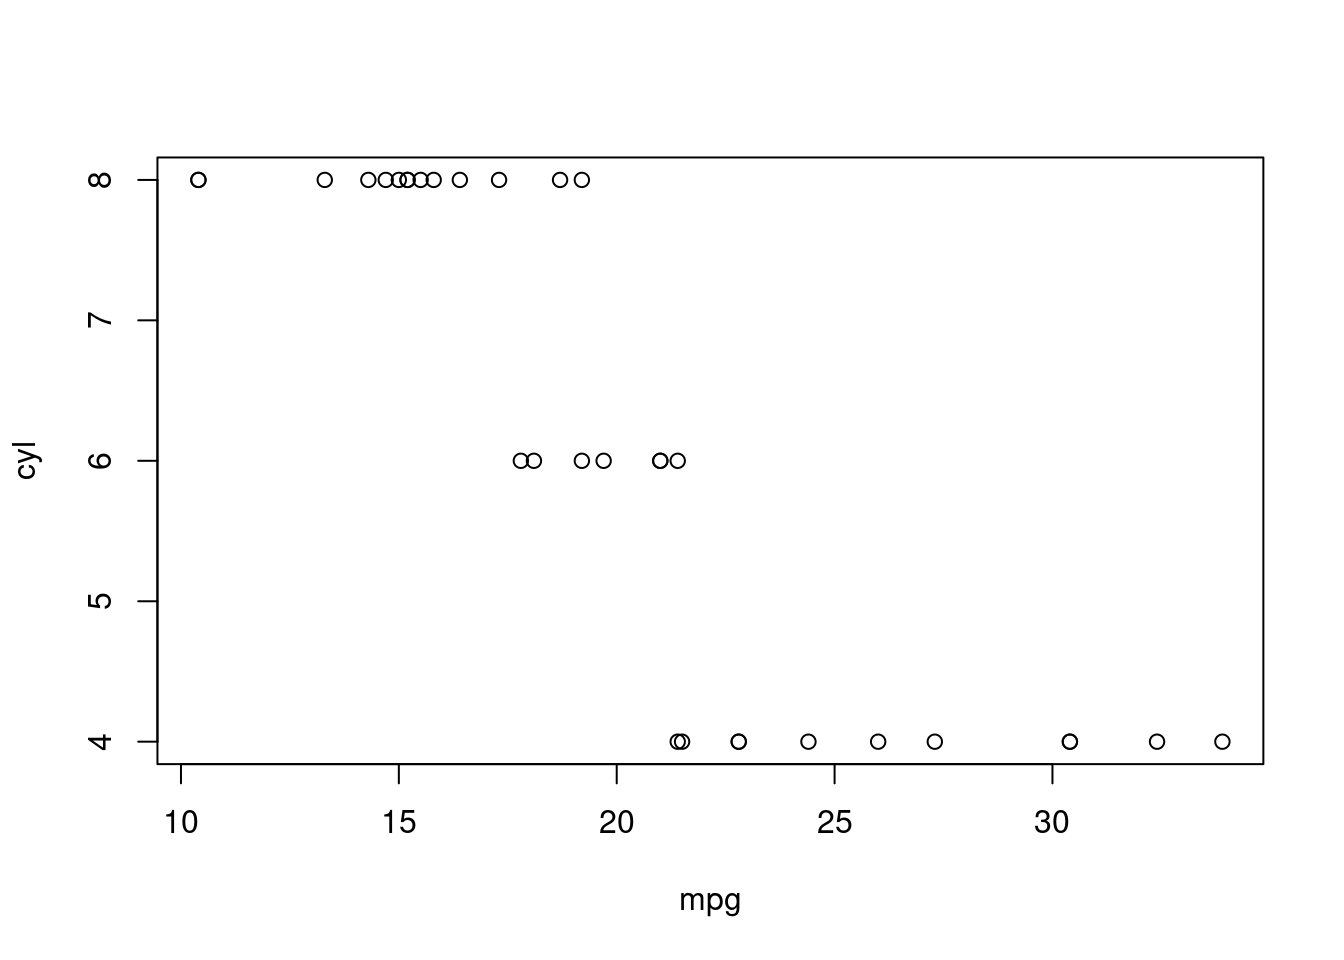
\includegraphics[width=0.8\linewidth]{Untitled_files/figure-latex/standard-plot-1} 

}

\caption{Great figure!}\label{fig:standard-plot}
\end{figure}

\begin{Shaded}
\begin{Highlighting}[]
\NormalTok{data <-}\StringTok{ }\NormalTok{iris}

\KeywordTok{plot}\NormalTok{(}\DataTypeTok{x =}\NormalTok{ data}\OperatorTok{$}\NormalTok{Sepal.Length, }
     \DataTypeTok{y =}\NormalTok{ data}\OperatorTok{$}\NormalTok{Sepal.Width, }
     \DataTypeTok{col =}\NormalTok{ data}\OperatorTok{$}\NormalTok{Species,}
     \DataTypeTok{pch =} \DecValTok{19}\NormalTok{, }
     \DataTypeTok{xlab =} \StringTok{"Sepal Length (cm)"}\NormalTok{,}
     \DataTypeTok{ylab =} \StringTok{"Sepal Width (cm)"}\NormalTok{)}
\end{Highlighting}
\end{Shaded}

\begin{figure}
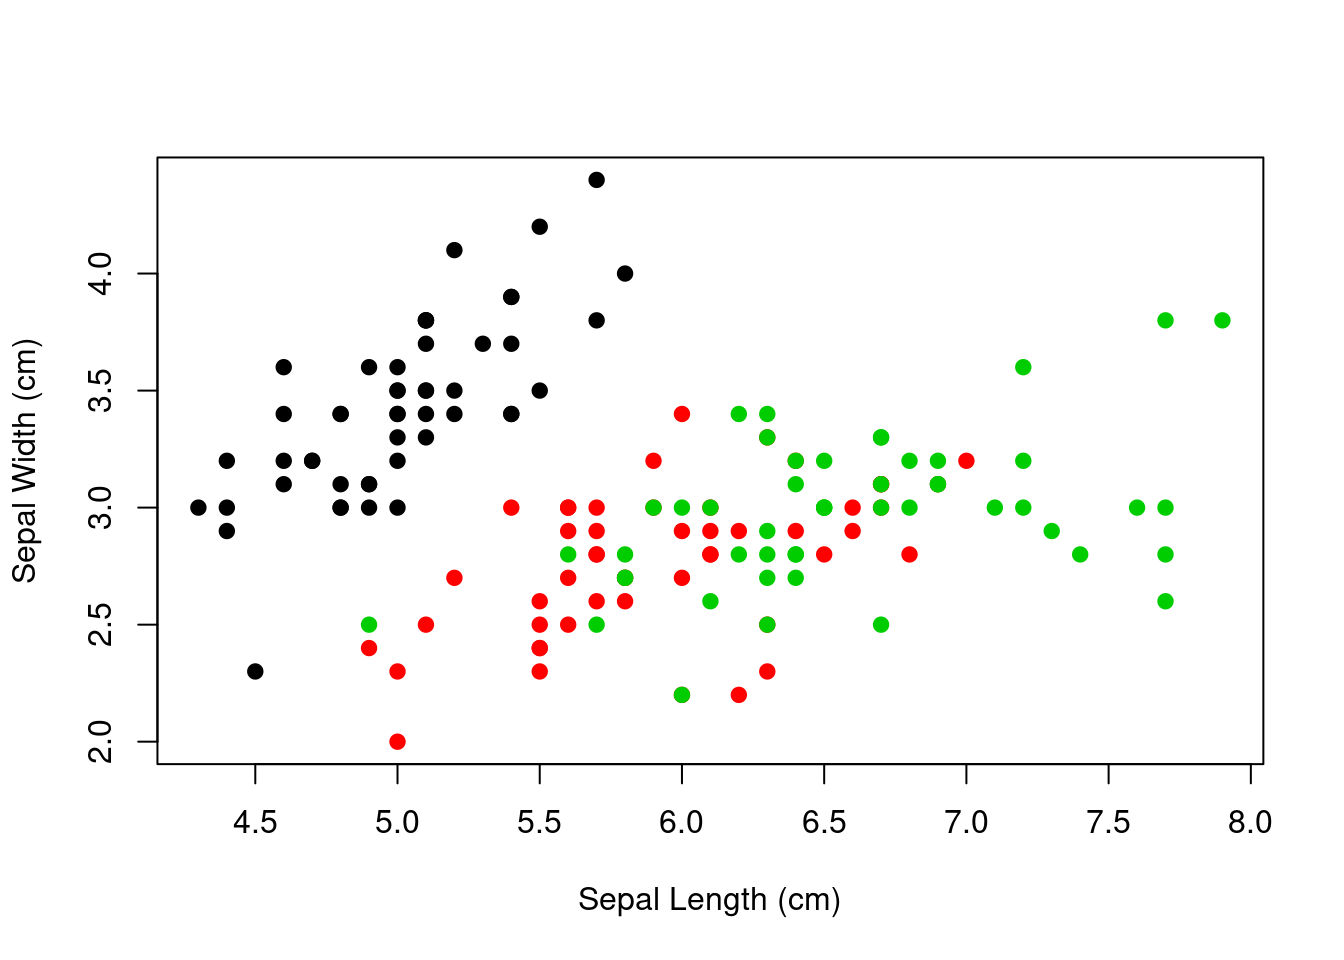
\includegraphics[width=0.8\linewidth]{Untitled_files/figure-latex/morefigs-1} \caption{Amazing, right?!}\label{fig:morefigs}
\end{figure}

\hypertarget{next-steps}{%
\section{Next Steps}\label{next-steps}}

Aliquam sed faucibus risus, quis efficitur erat. Vestibulum semper
mauris quis tempus eleifend. Aliquam sagittis dictum ipsum, quis viverra
ligula eleifend ut. Curabitur sagittis vitae arcu eget faucibus. In non
elementum felis. Duis et aliquam nunc. Nunc pulvinar sapien nunc, vel
pretium nisi efficitur in. Fusce fringilla maximus leo et maximus. Fusce
at ligula laoreet, iaculis mi at, auctor odio. Praesent sed elementum
justo. Aenean consectetur risus rhoncus tincidunt efficitur. Praesent
dictum mauris at diam maximus maximus (Thorne 2019).

\hypertarget{conclusion}{%
\section{Conclusion}\label{conclusion}}

Try \texttt{posterdown} out! Hopefully you like it!

\hypertarget{references}{%
\section*{References}\label{references}}
\addcontentsline{toc}{section}{References}

\hypertarget{refs}{}
\leavevmode\hypertarget{ref-R-rmarkdown}{}%
Allaire, JJ, Yihui Xie, Jonathan McPherson, Javier Luraschi, Kevin
Ushey, Aron Atkins, Hadley Wickham, Joe Cheng, Winston Chang, and
Richard Iannone. 2020. \emph{Rmarkdown: Dynamic Documents for R}.
\url{https://CRAN.R-project.org/package=rmarkdown}.

\leavevmode\hypertarget{ref-R-posterdown}{}%
Thorne, Brent. 2019. \emph{Posterdown: Generate Pdf Conference Posters
Using R Markdown}. \url{https://CRAN.R-project.org/package=posterdown}.

\leavevmode\hypertarget{ref-R-pagedown}{}%
Xie, Yihui, Romain Lesur, Brent Thorne, and Xianying Tan. 2020.
\emph{Pagedown: Paginate the Html Output of R Markdown with Css for
Print}. \url{https://CRAN.R-project.org/package=pagedown}.

\end{document}
